Ce qui suit tente de donner une explication naturelle du lien entre la loi $\star$ et un procédé géométrique rappelé par Jérôme Germoni précédemment cité.


\bigskip

Jusqu'à présent, nous n'avons à aucun moment représenter l'hyperbole $\geoset{H}$ \squote{à deux branches} d'équation implicite $X^2 - 8 Y^2 = 1$ \textit{(on utilise ici des majuscules pour le système de coordonnées)}. C'est un peu dommage !


\medskip

Ci-dessous se trouvent quatre représentations avec deux points $M$ et $N$ sur $\geoset{H}$ de coordonnées respectives 
$\begin{pmatrix}
  x \\ 
  y 
\end{pmatrix}$
et
$\begin{pmatrix} 
  x' \\ 
  y' 
\end{pmatrix}$
ainsi que les points $E$ , cf. le neutre de $\star$ , et $P$, eux aussi sur $\geoset{H}$ , de coordonnées respectives 
$\begin{pmatrix}
  1 \\ 
  0 
\end{pmatrix}$
et
$\begin{pmatrix} 
  x'' \\ 
  y''
\end{pmatrix}
=
\begin{pmatrix}
  x \\ 
  y 
\end{pmatrix}
\star
\begin{pmatrix} 
  x' \\ 
  y'
\end{pmatrix}$ .


\bigskip


\begin{multicols}{2}
	\center
	
	\fbox{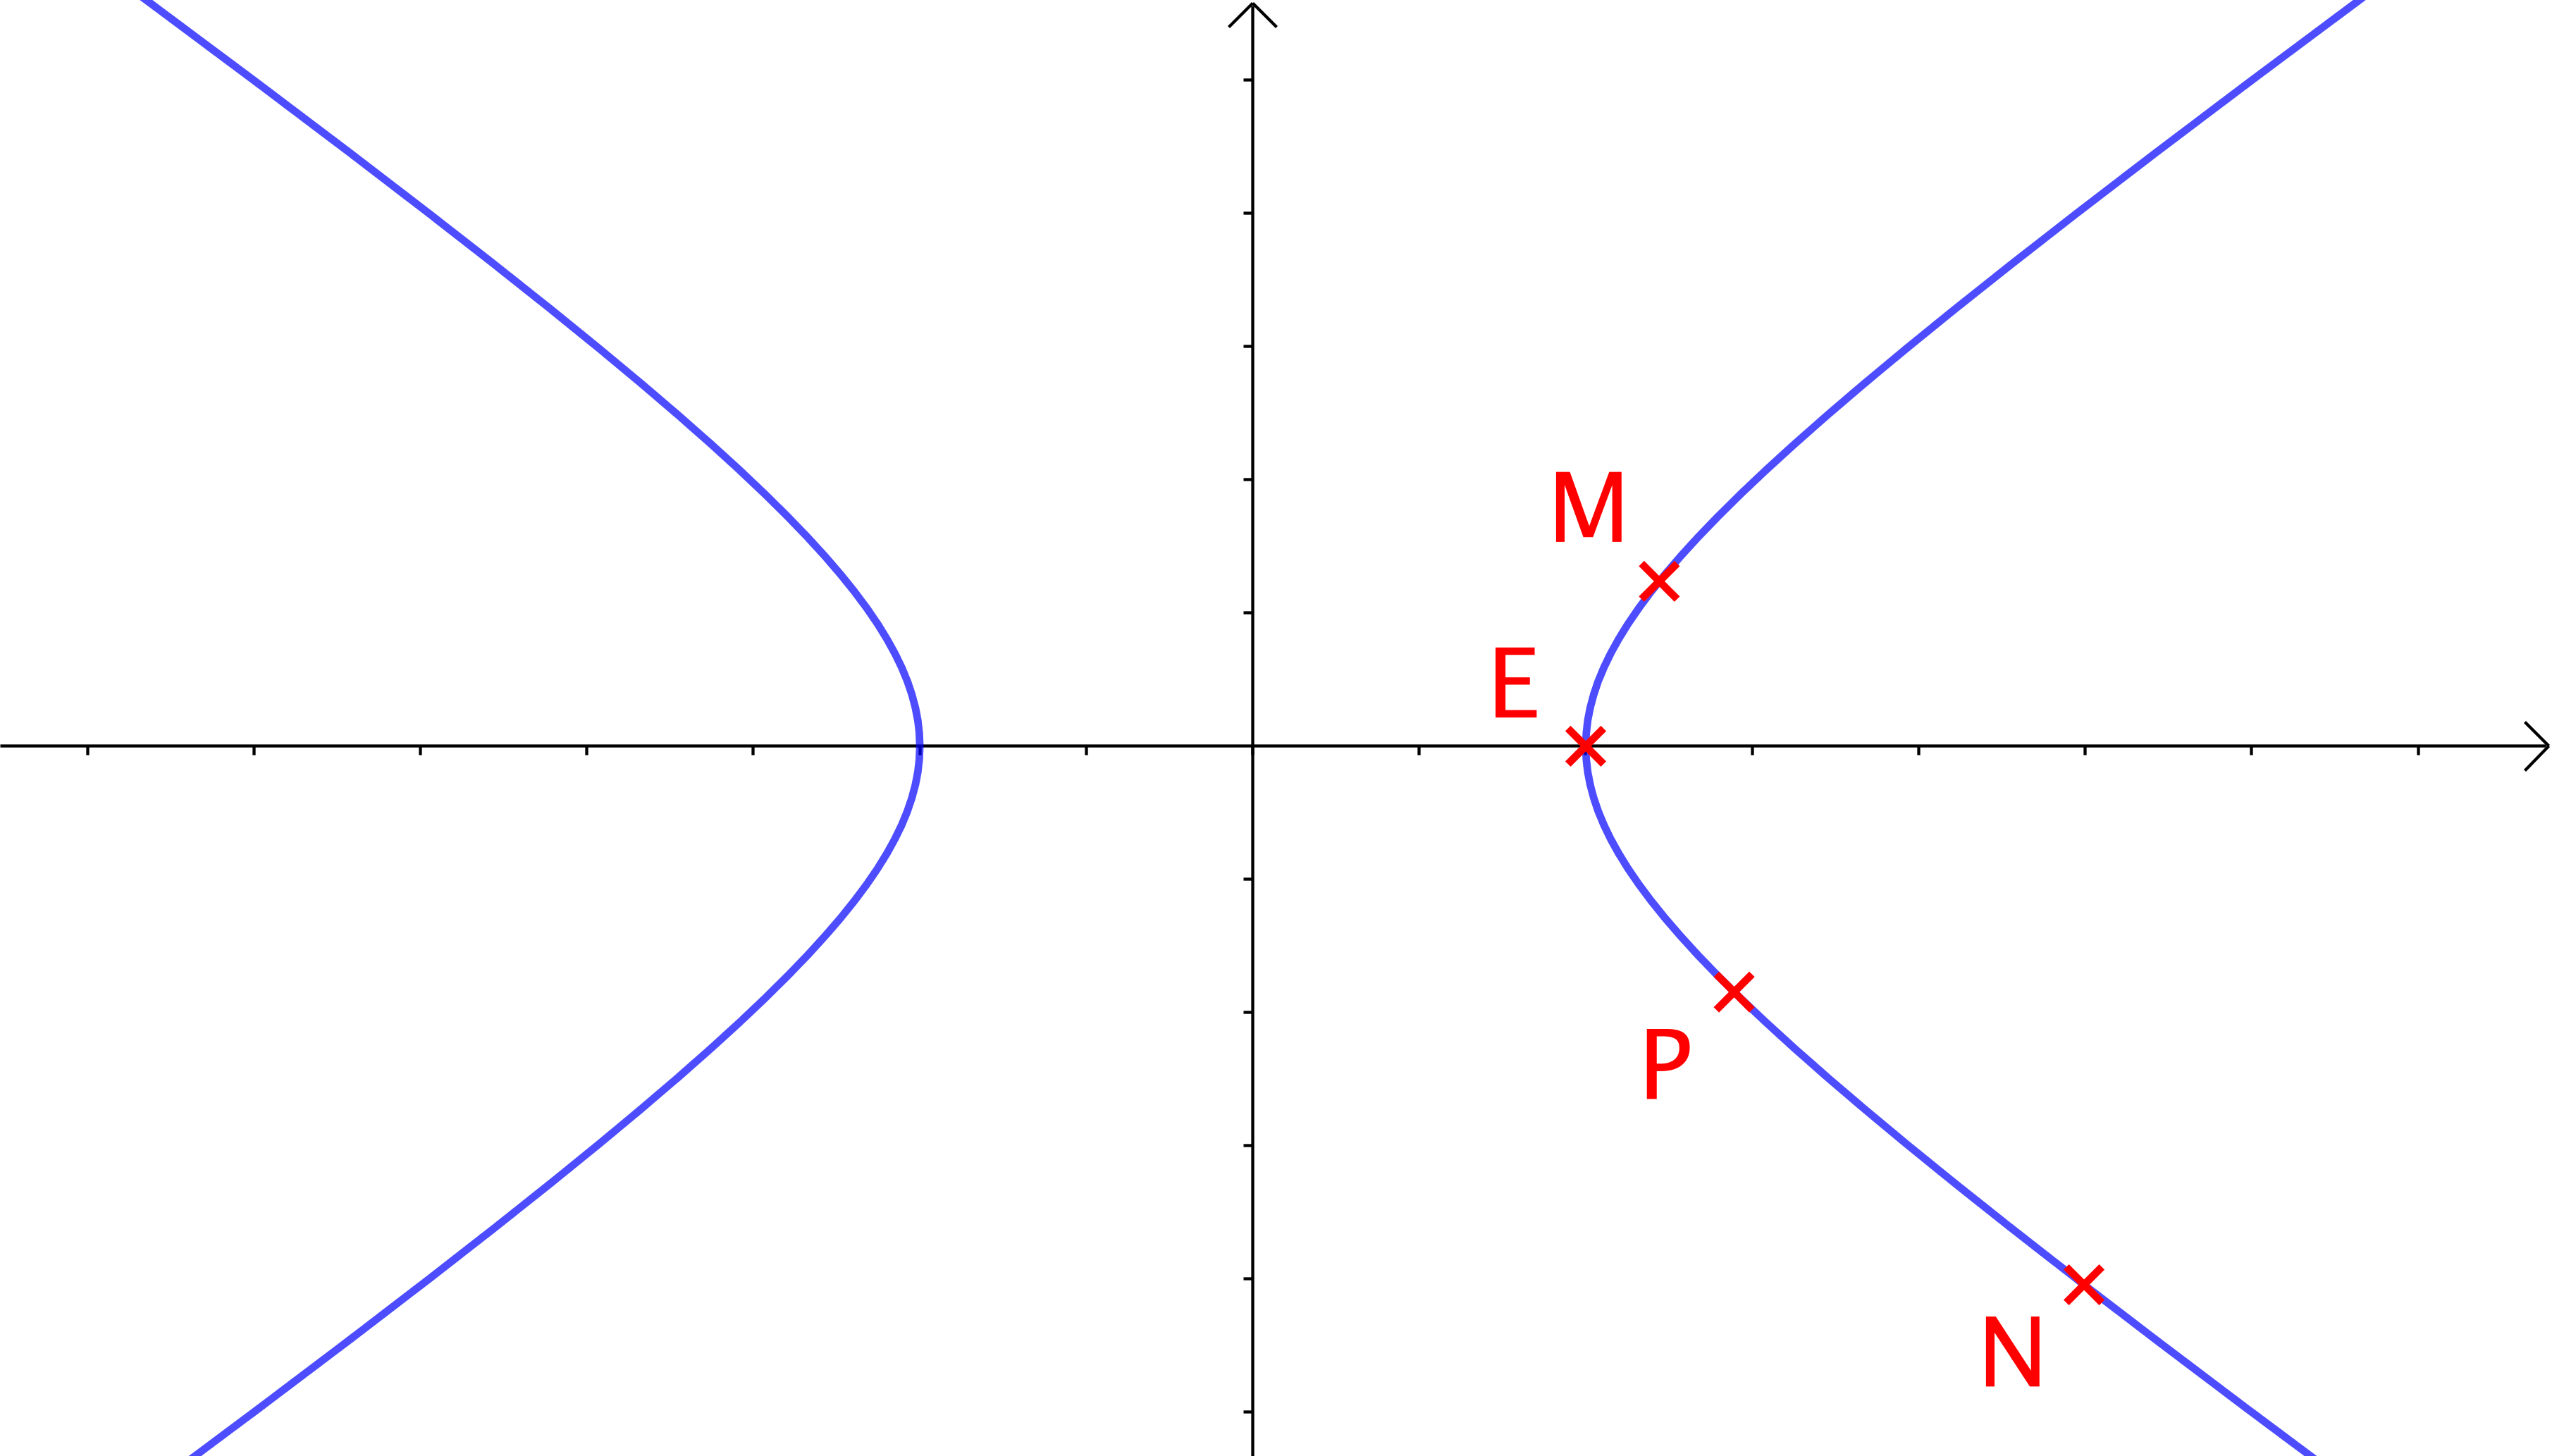
\includegraphics[scale = .5]{exo-spe-math-bac-s-juin-2018/geometry-is-the-queen/oblic-1.png}}
	
	\bigskip
	
	\fbox{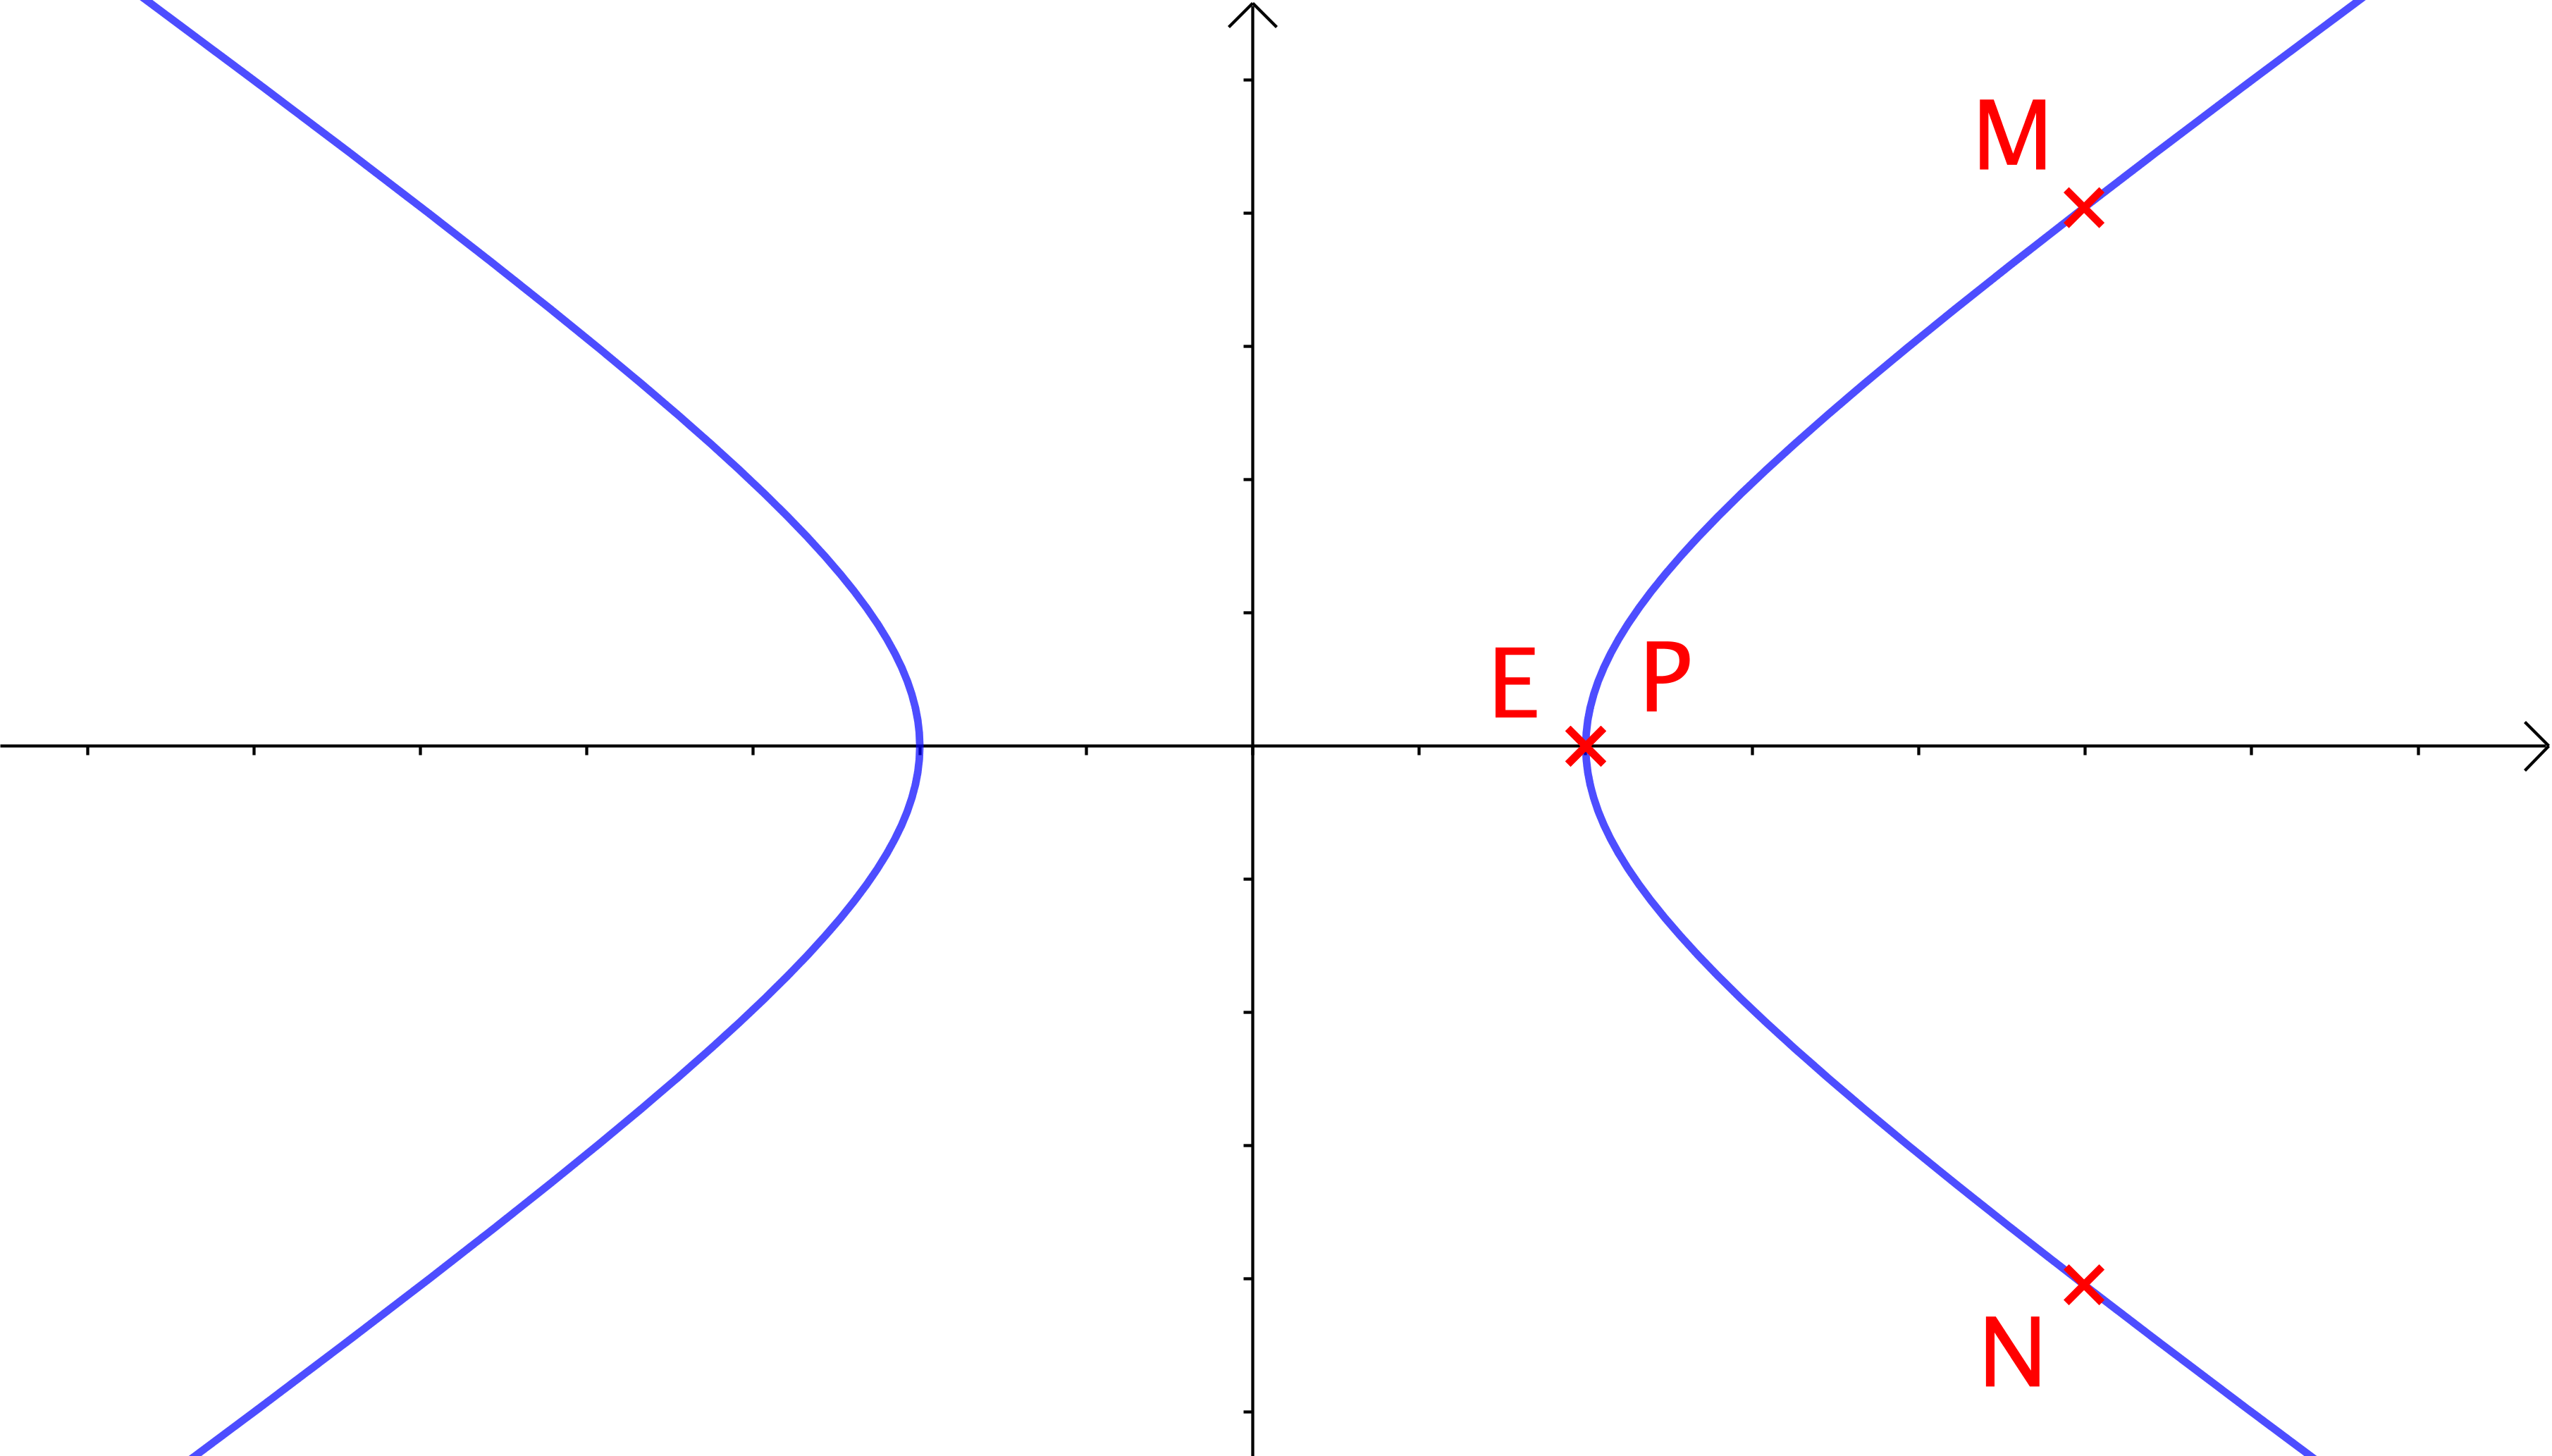
\includegraphics[scale = .5]{exo-spe-math-bac-s-juin-2018/geometry-is-the-queen/vertical-case.png}}

	\columnbreak
	
	\fbox{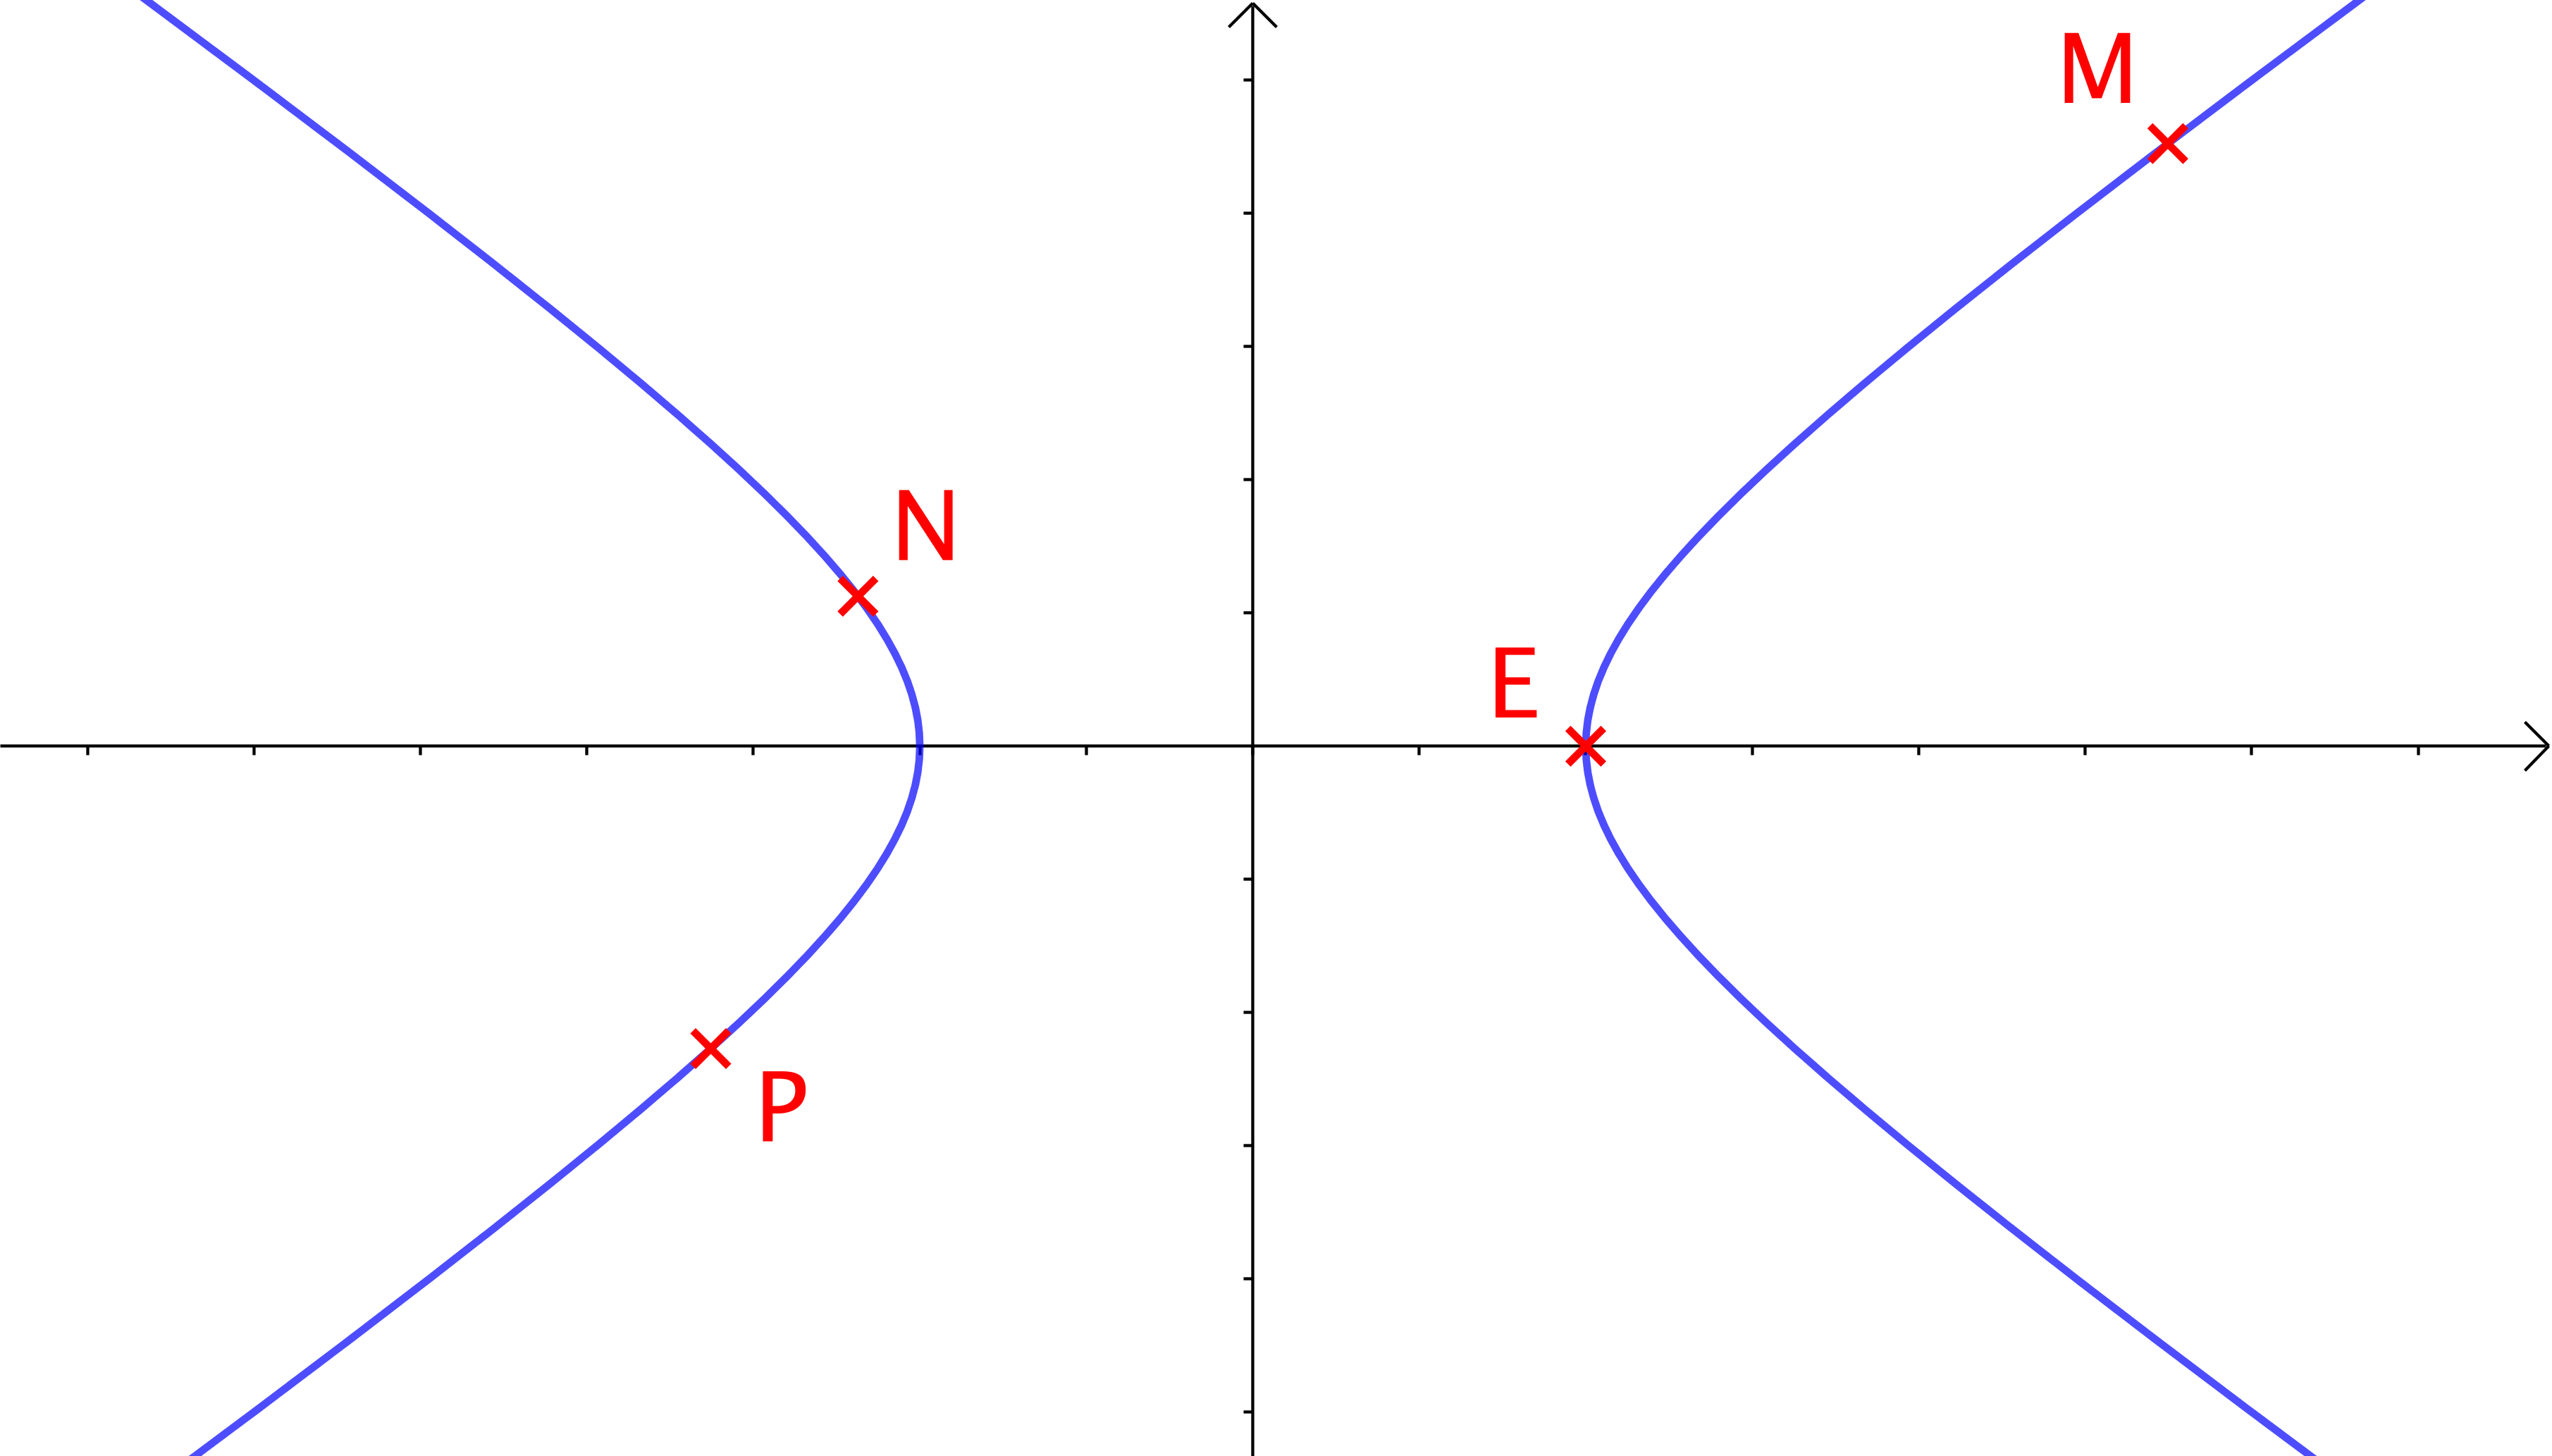
\includegraphics[scale = .5]{exo-spe-math-bac-s-juin-2018/geometry-is-the-queen/oblic-2.png}}
	
	\bigskip

	\fbox{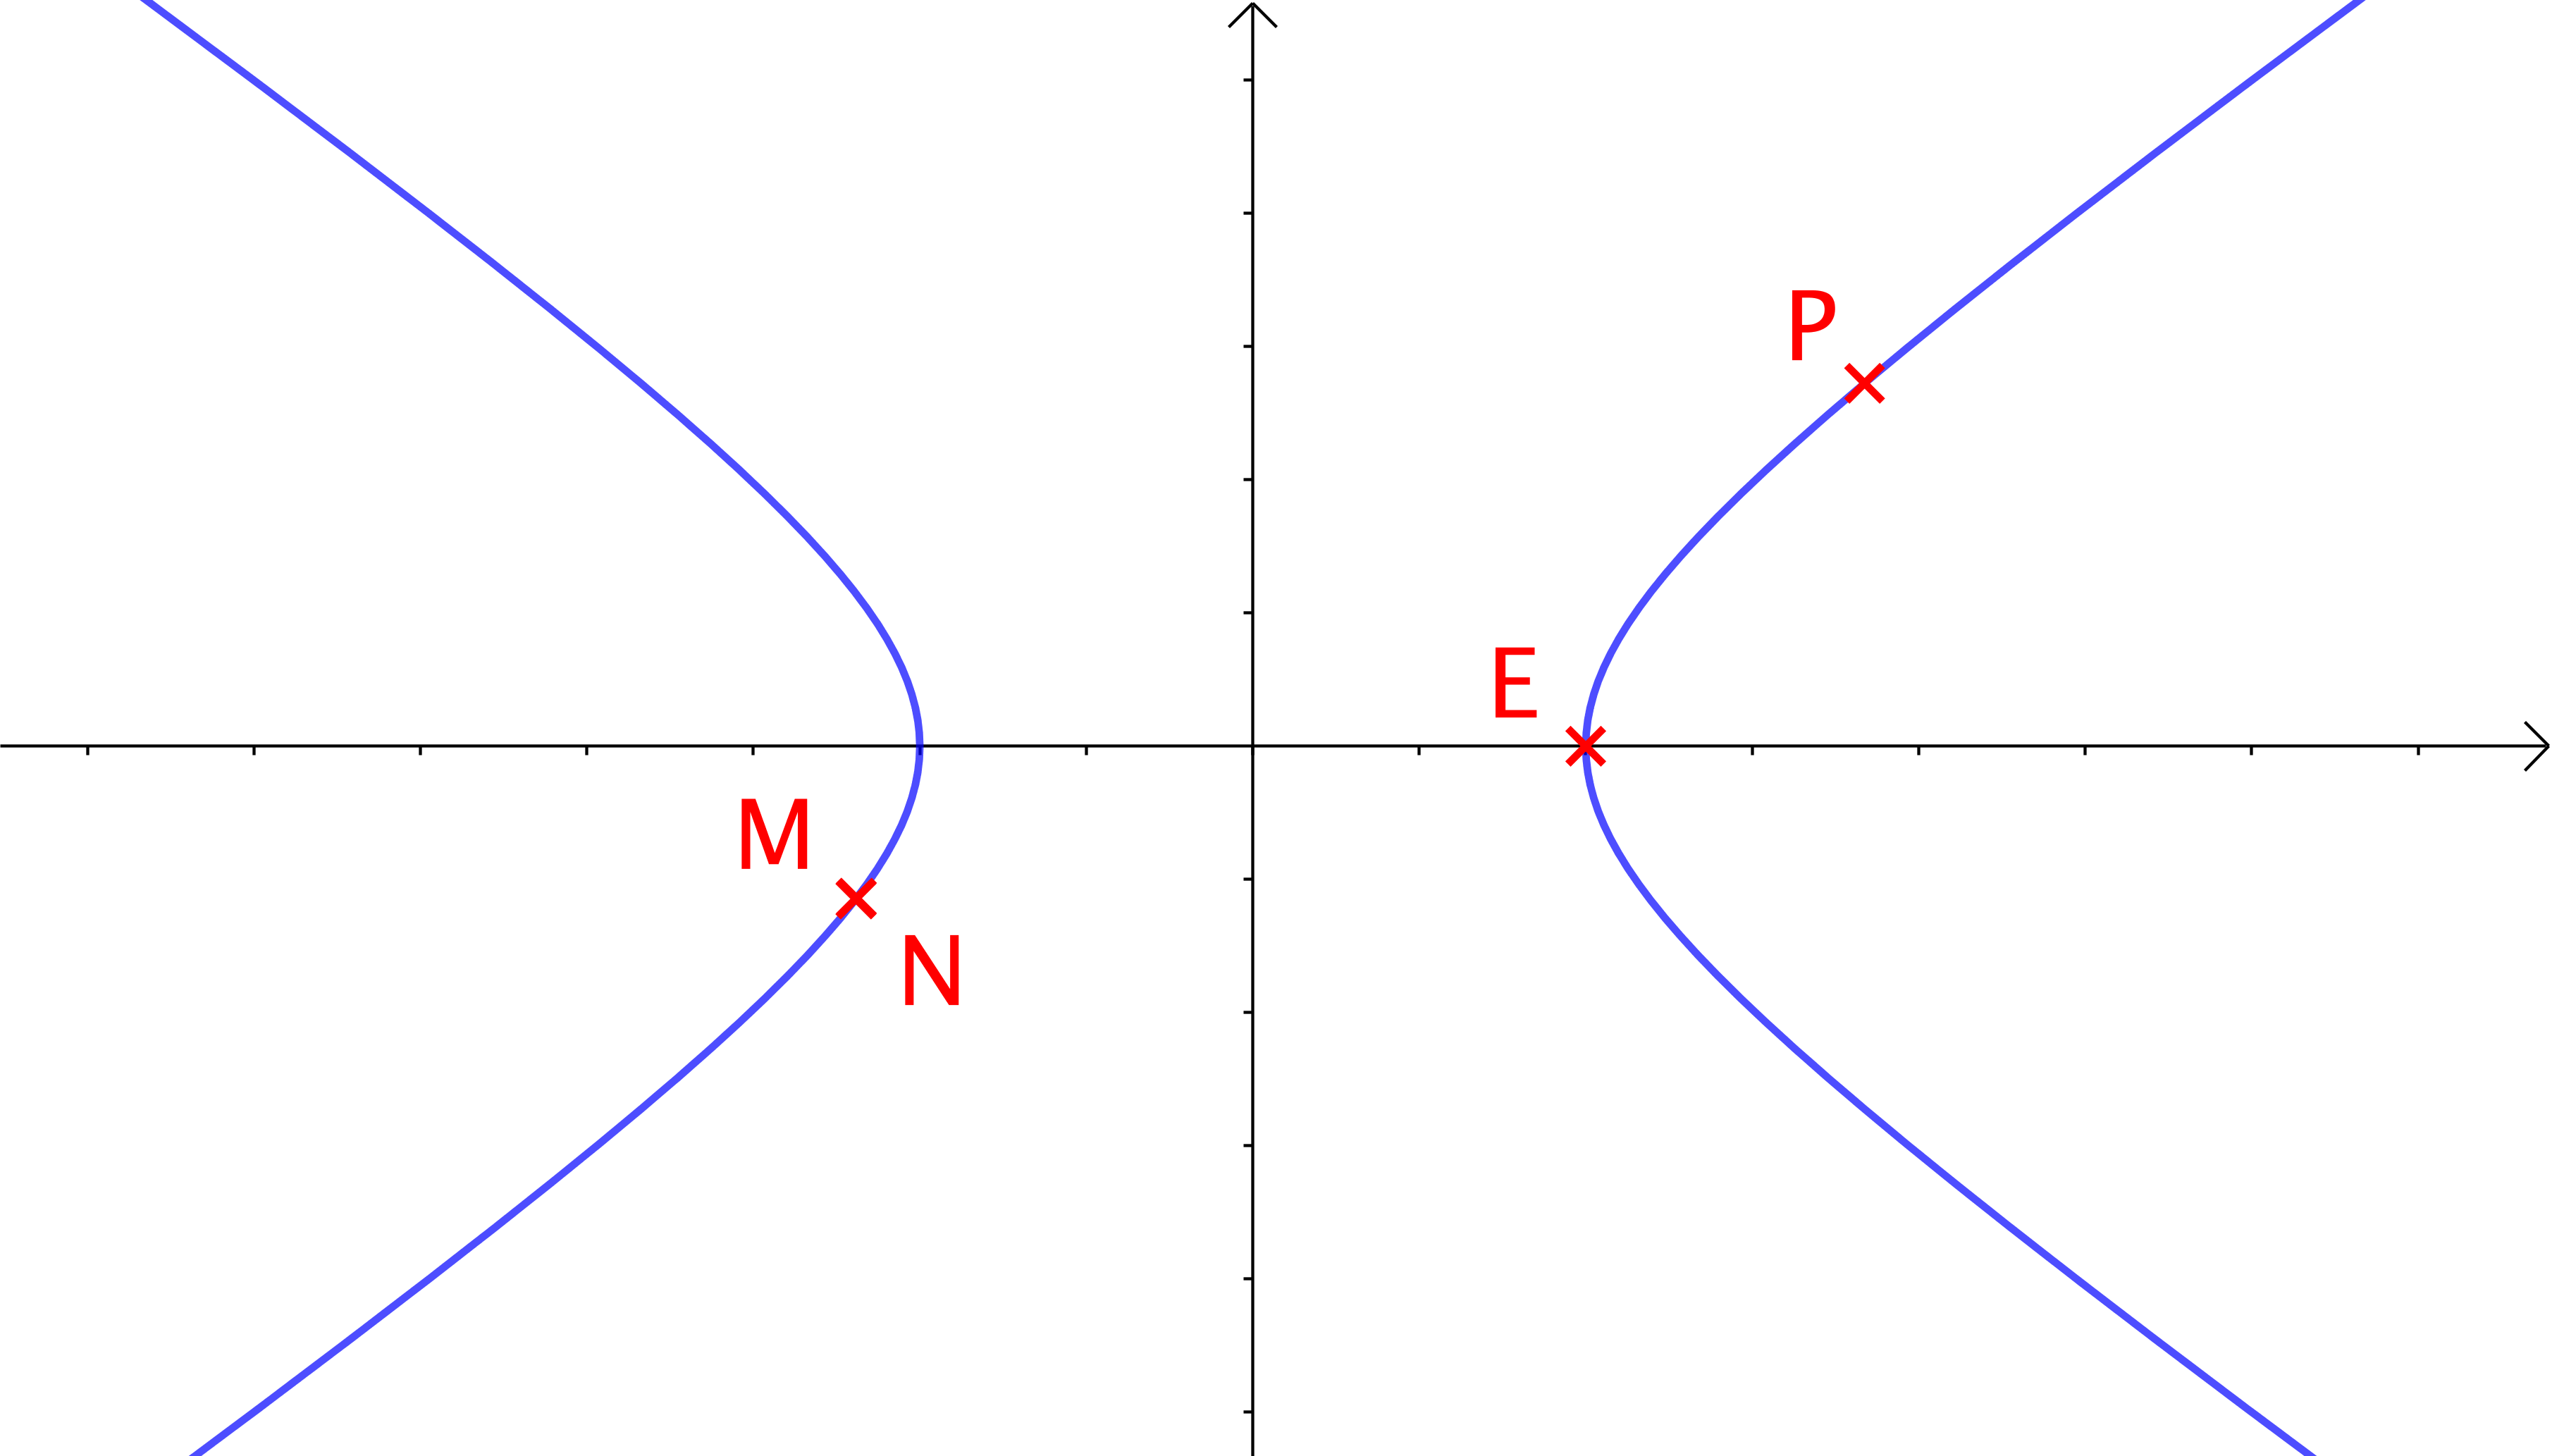
\includegraphics[scale = .5]{exo-spe-math-bac-s-juin-2018/geometry-is-the-queen/same-points.png}}
\end{multicols}


\bigskip
	

Les graphiques précédents suggèrent
\footnote{
	Le lieu de téléchargement de ce document contient un fichier GeoGebra \texttt{base-tool.ggb} manipulable dynamiquement pour vérifier combien il est aisé de conjecturer la construction géométrique.
}
un procédé géométrique simple pour construire $P$.

\begin{enumerate}
	\item Si $M \neq N$ et $x_M \neq x_N$ alors on construit la parallèle à $(MN)$ passant par $E$ . Le point $P$ est le second point d'intersection de cette parallèle avec $\geoset{H}$ \emph{(notons qu'une droite coupe $\geoset{H}$ en au plus deux points)}.


	\item Si $M \neq N$ et $x_M = x_N$ alors $P = E$ . Notons au passage que l'on peut voir ceci comme un cas limite du précédent avec un point d'intersection \squote{double}.


	\item Si $M = N$ on procède comme ci-dessus mais avec la parallèle de la tangente à $\geoset{H}$ au point $M$ .
\end{enumerate}


Dans les graphiques suivants, nous avons tracé les droites utilisées par le procédé géométrique conjecturé à l'instant.


\medskip


\begin{multicols}{2}
	\center
	
	\fbox{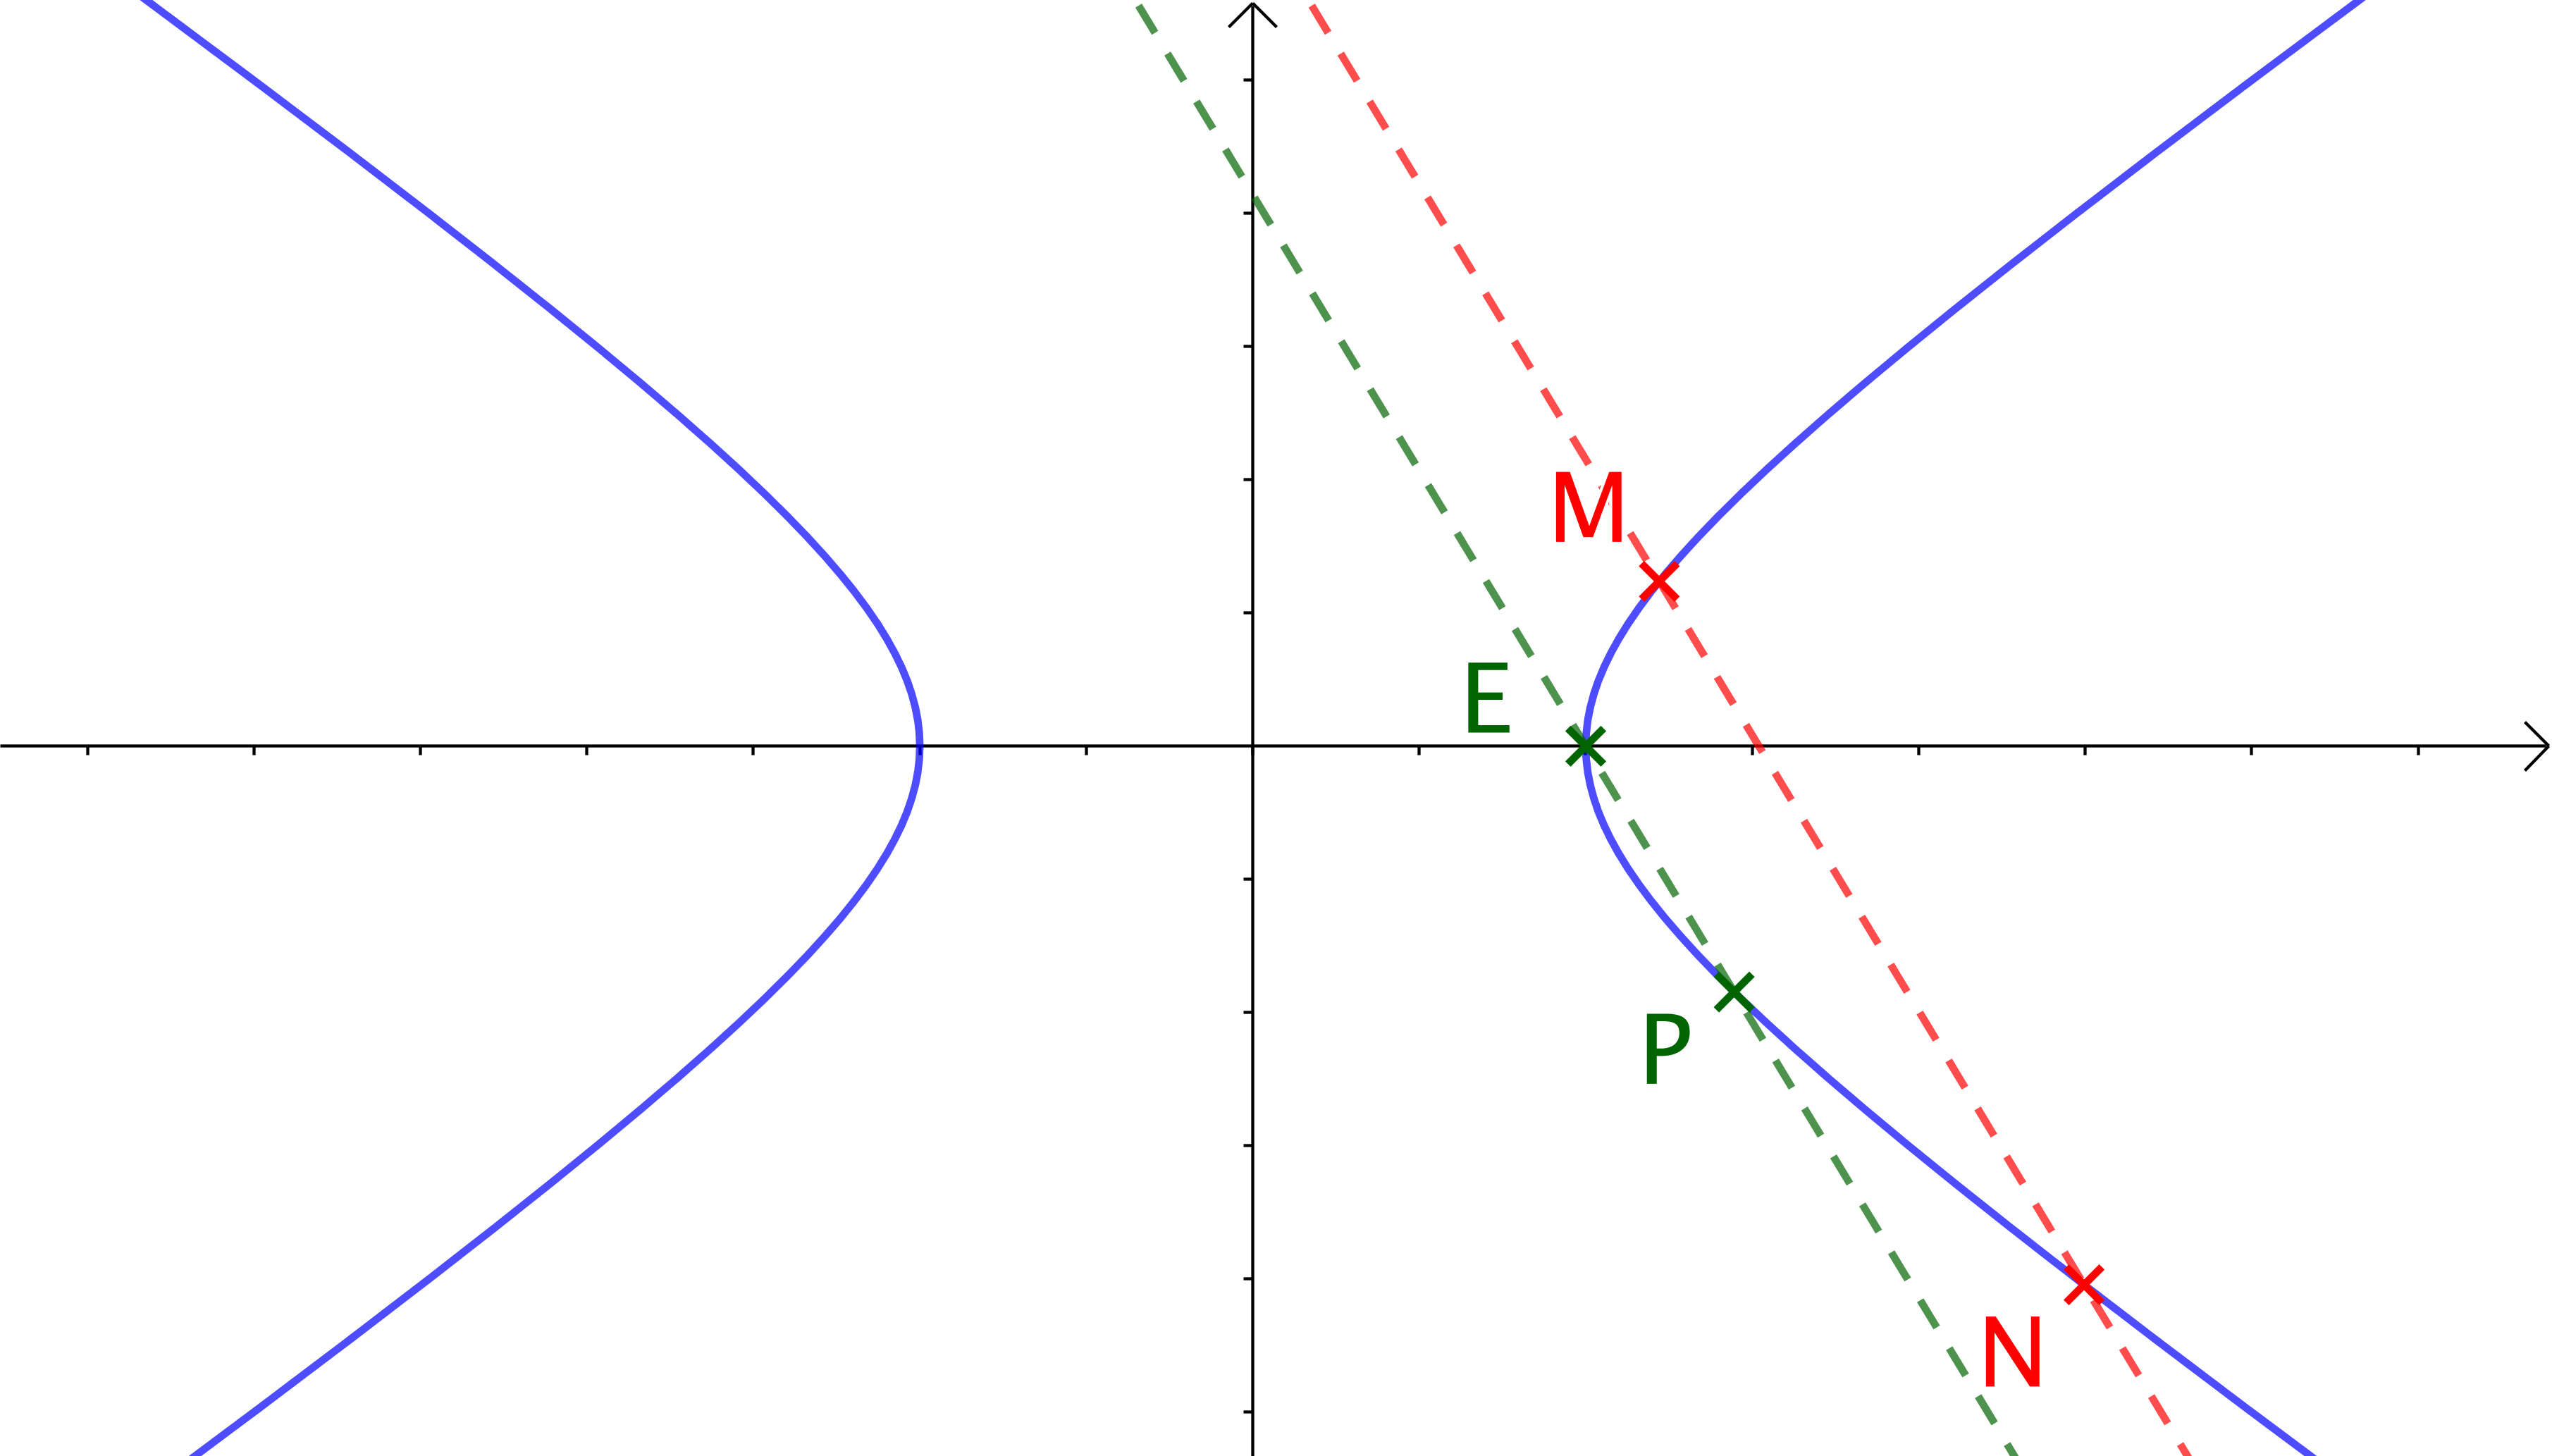
\includegraphics[scale = .5]{exo-spe-math-bac-s-juin-2018/geometry-is-the-queen/oblic-1-with-lines.png}}
	
	\bigskip
	
	\fbox{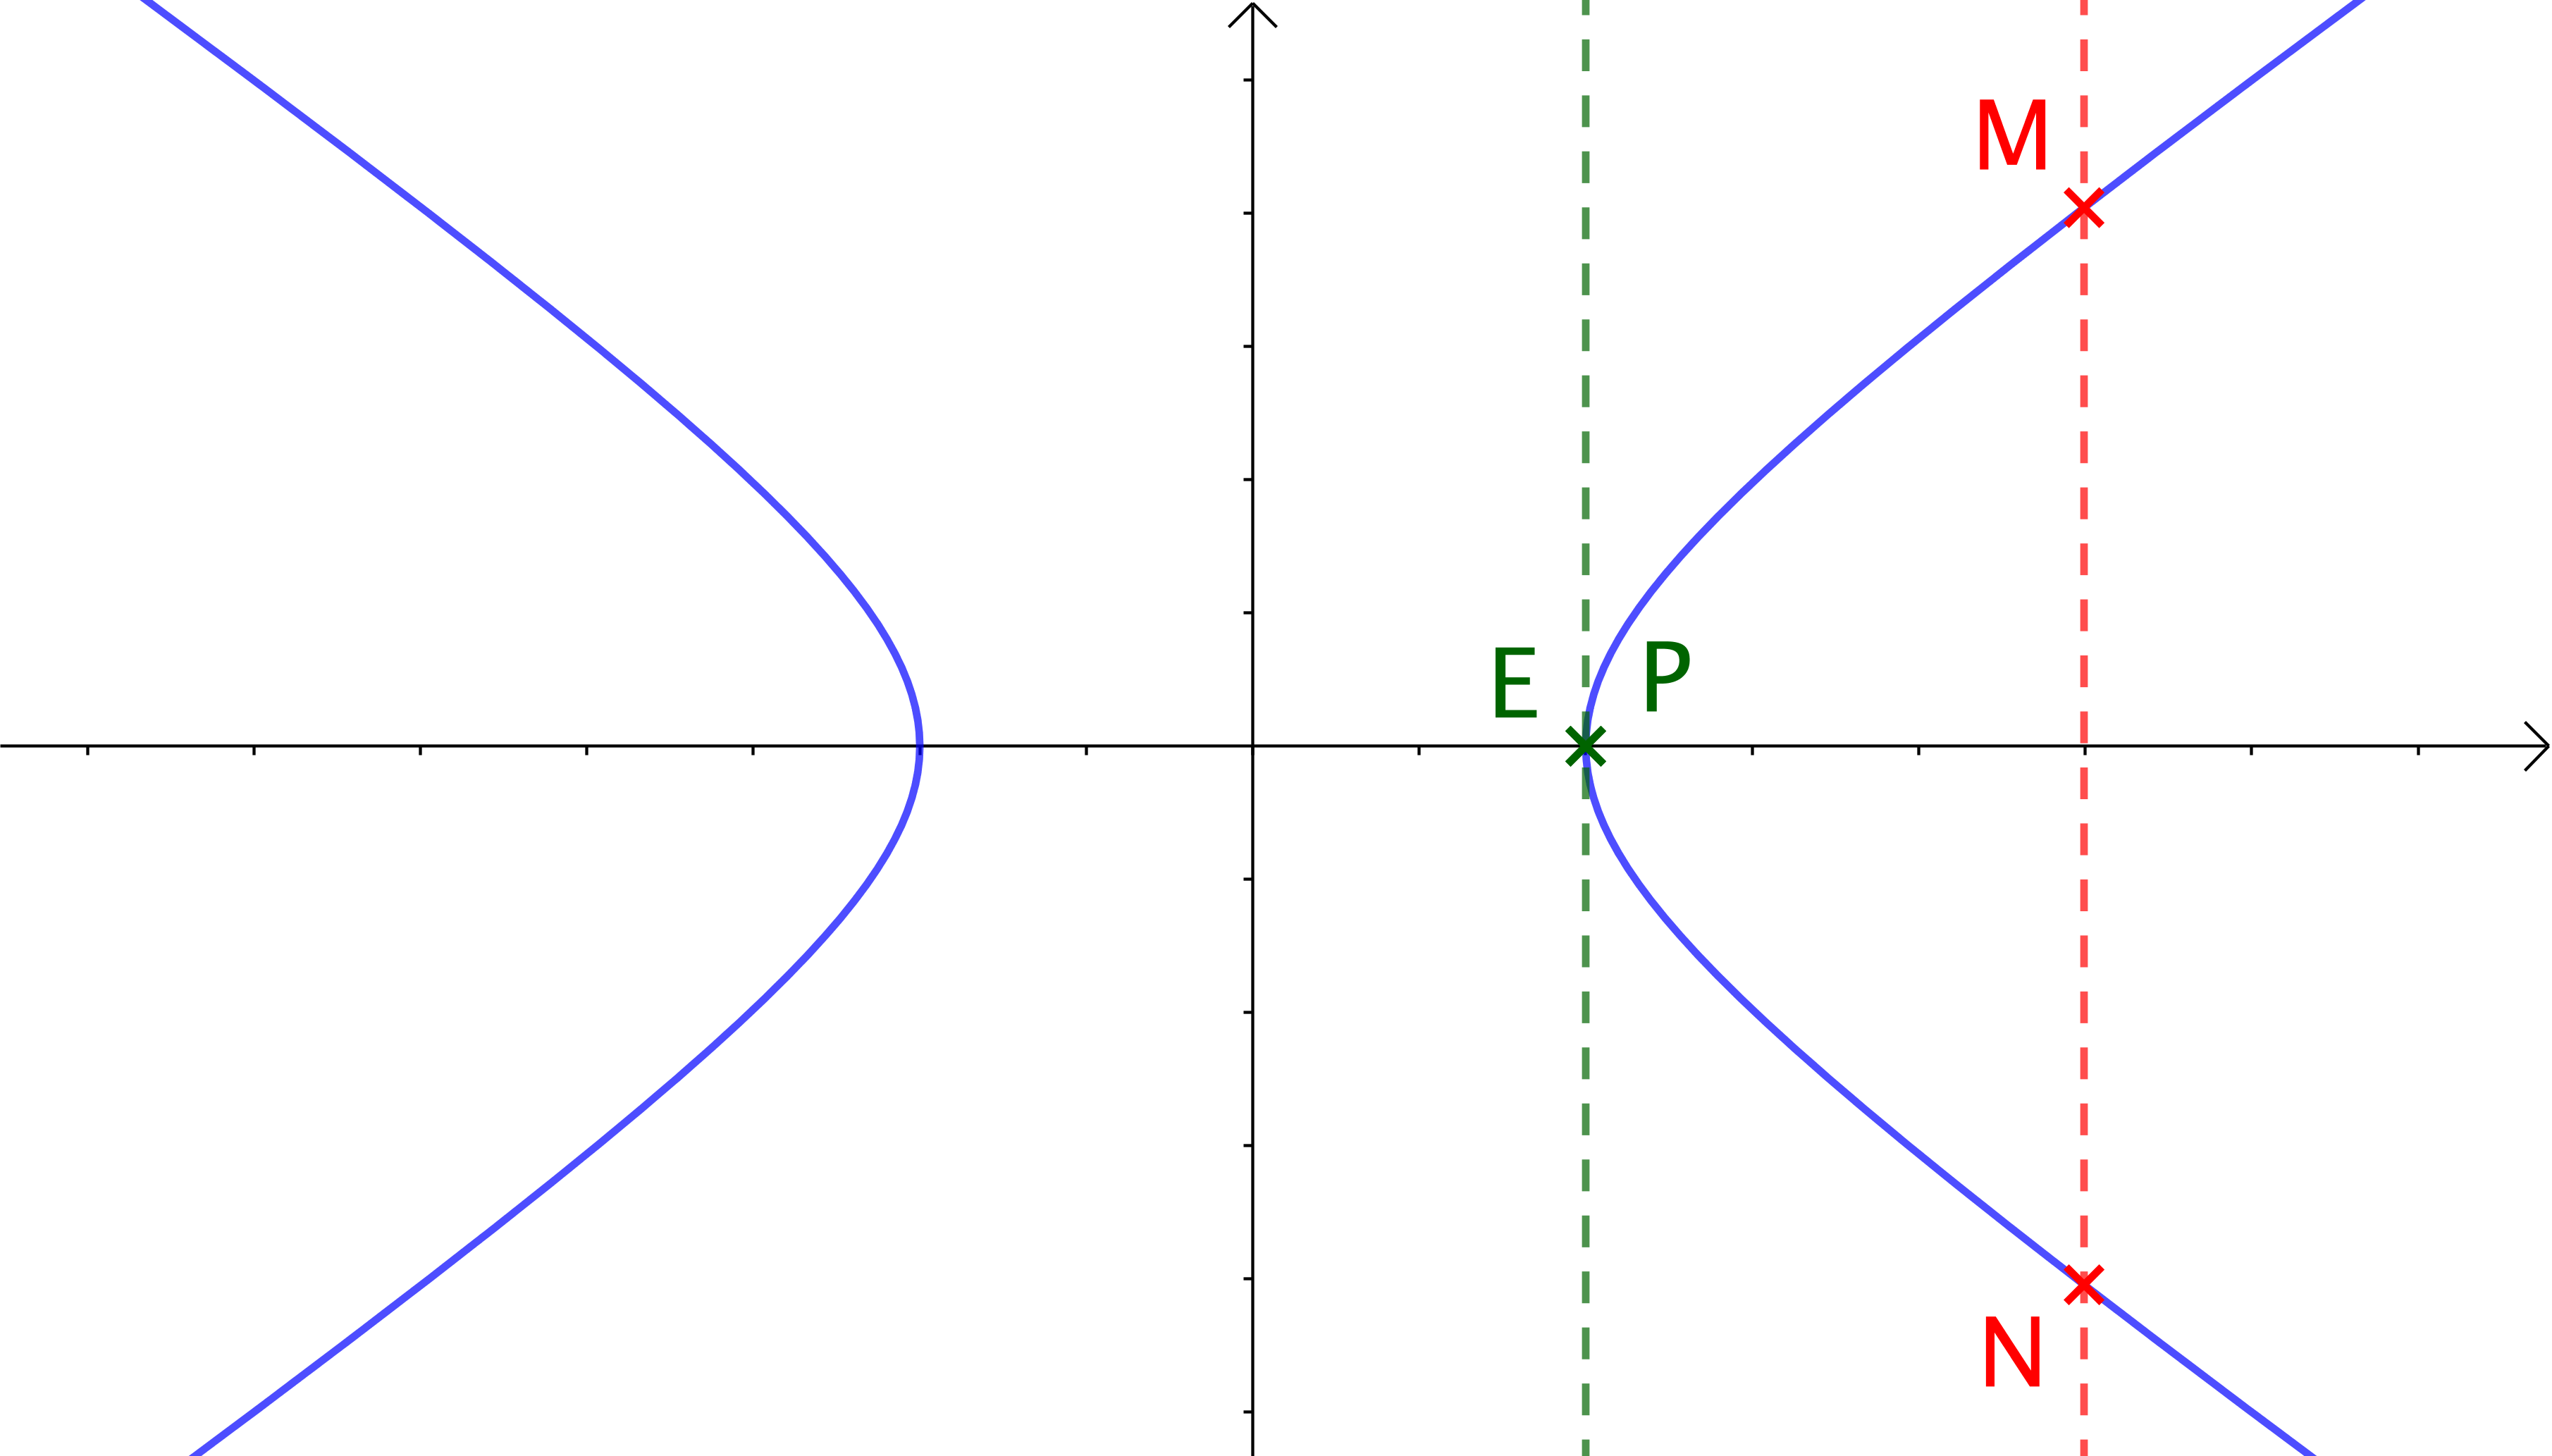
\includegraphics[scale = .5]{exo-spe-math-bac-s-juin-2018/geometry-is-the-queen/vertical-case-with-lines.png}}

	\columnbreak
	
	\fbox{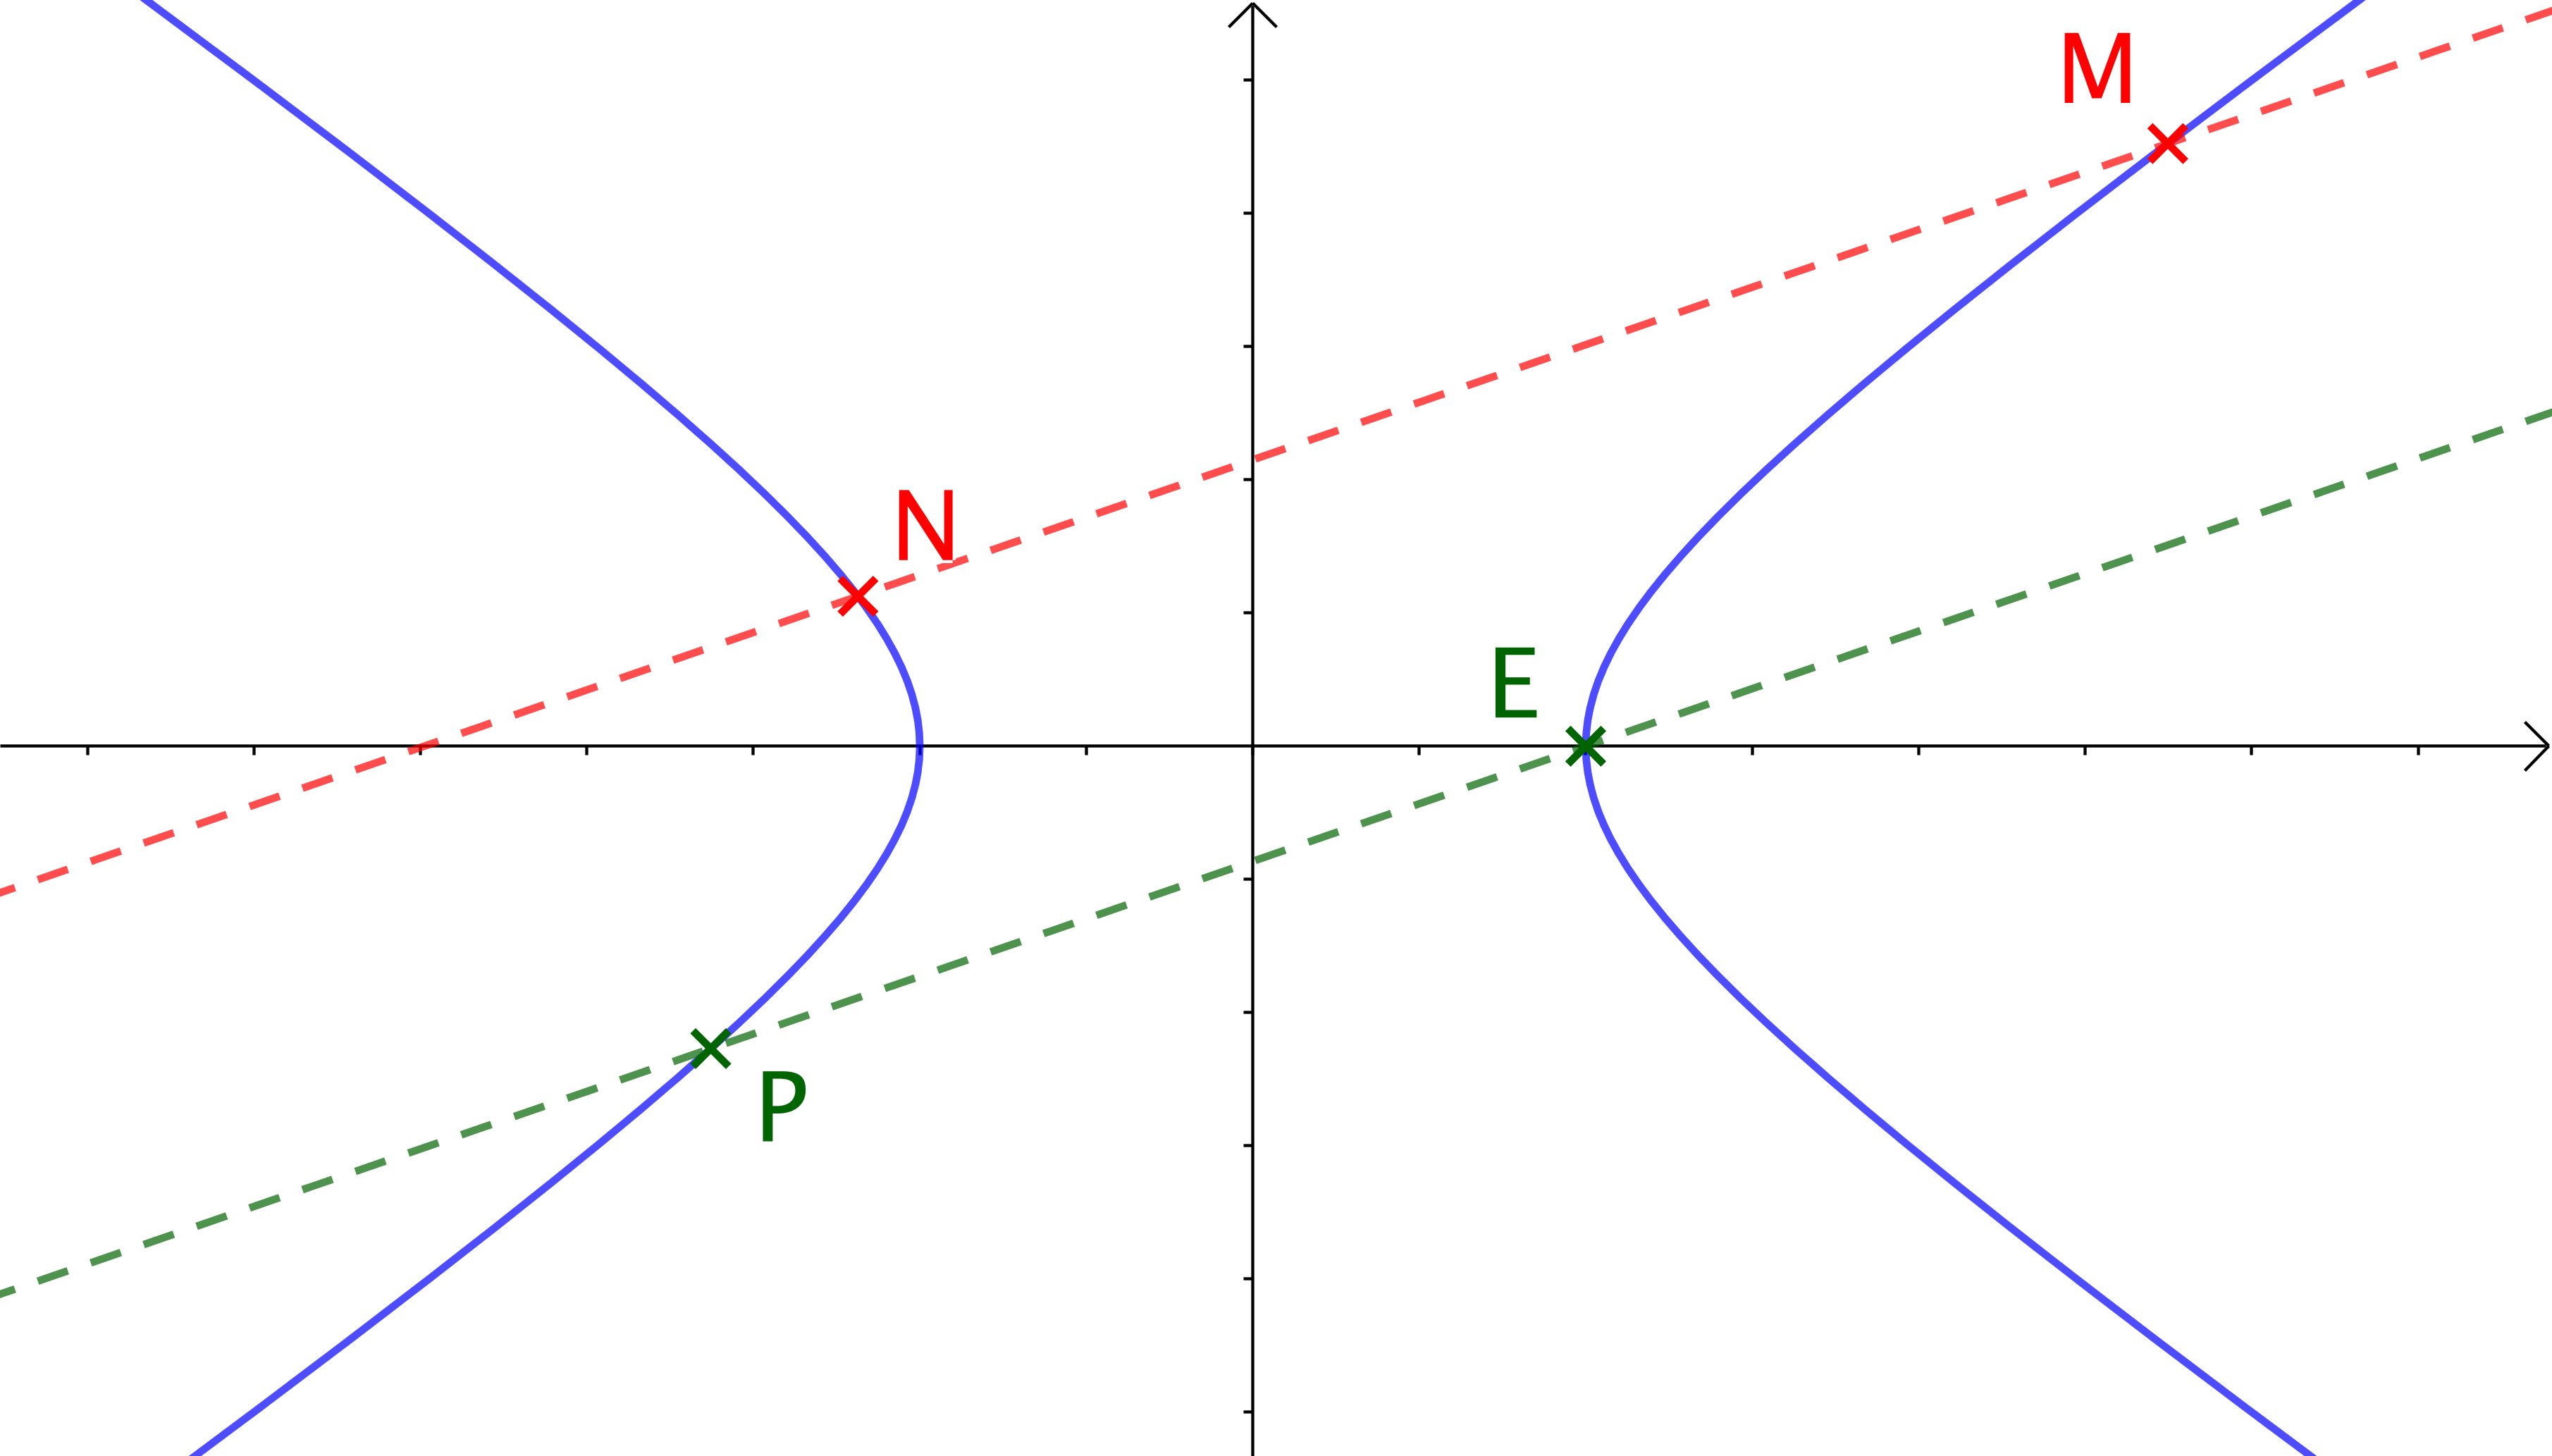
\includegraphics[scale = .5]{exo-spe-math-bac-s-juin-2018/geometry-is-the-queen/oblic-2-with-lines.png}}
	
	\bigskip

	\fbox{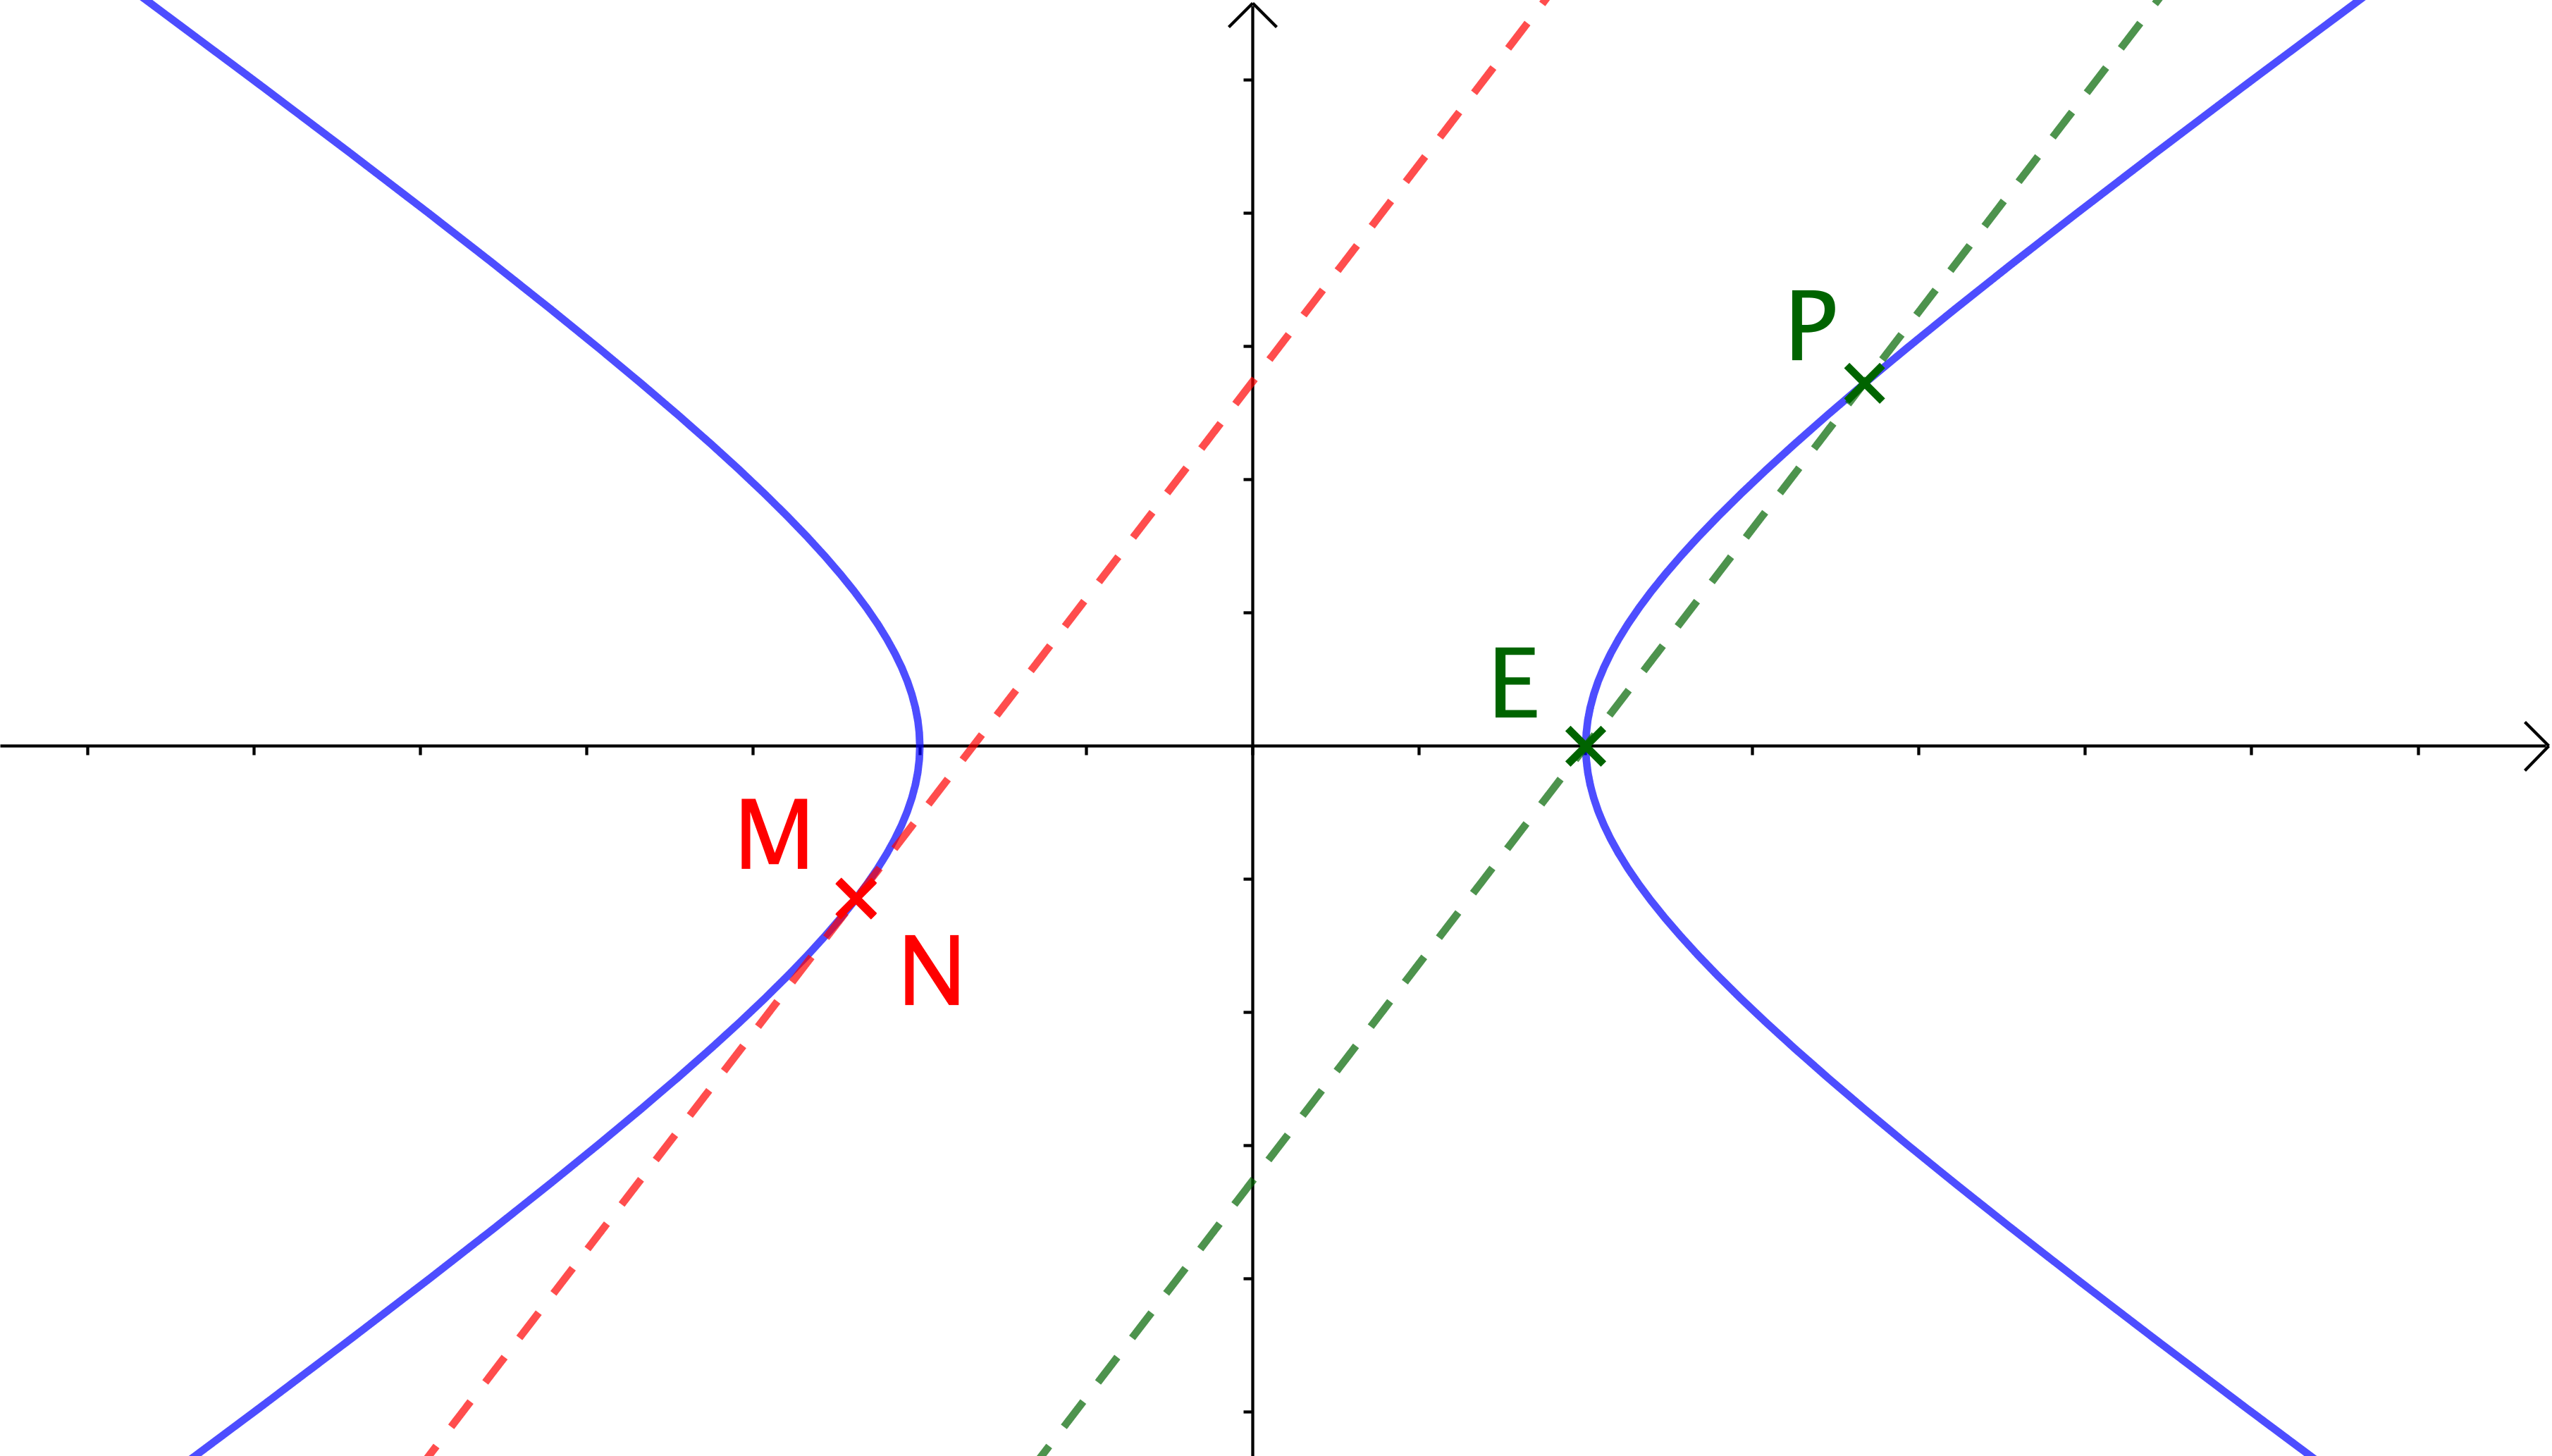
\includegraphics[scale = .5]{exo-spe-math-bac-s-juin-2018/geometry-is-the-queen/same-points-with-lines.png}}
\end{multicols}


\bigskip

Prouvons la validité de notre conjecture. Nous confondrons les points avec les vecteurs utilisés pour définir la loi $\star$ .

\begin{enumerate}
	\item Supposons que $M \neq N$ avec $x_M \neq x_N$ .
	
	\smallskip
	
	\noindent
	Nous devons juste vérifier que $(EP)$ et $(MN)$ sont parallèles puisque l'on sait que $P \neq E$ \textit{(voir le point suivant si besoin)}. Ce qui suit est quelque peu brutal \textit{(on pourrait faire appel à un logiciel de calcul formel qui ici peut être utilisé en toute confiance)}.
	
	\smallskip
	
	\noindent
	$\det\left ( \vect{EP} ; \vect{MN} \right)
	=
	\left|\begin{NiceArray}{CC} 
	  x'' - 1 & x' - x \\ 
	  y''     & y' - y
	\end{NiceArray}\right|$
	
	\noindent
	$\phantom{\det\left ( \vect{EP} ; \vect{MN} \right)}
	=
	(x'' - 1)(y' - y) -  y'' (x' - x)$
	
	\noindent
	$\phantom{\det\left ( \vect{EP} ; \vect{MN} \right)}
	=
	(x x' + 8 y y' - 1)(y' - y) -  (y x' + x y') (x' - x)$
	
	\noindent
	$\phantom{\det\left ( \vect{EP} ; \vect{MN} \right)}
	=
	x x' y' + 8 y y'^2 - y' - x x' y - 8 y^2 y' + y
	- 
	y x'^2 - x x' y' + y x x' + x^2 y'$
	
	\noindent
	$\phantom{\det\left ( \vect{EP} ; \vect{MN} \right)}
	=
	8 y y'^2 - y' - 8 y^2 y' + y
	- 
	y x'^2 + x^2 y'$
	
	\smallskip
	
	\noindent
	Réordonnons les termes en nous souvenant que $x^2 - 8 y^2 = 1$ et $x'^2 - 8 y'^2 = 1$ .

	\smallskip
	
	\noindent
	${\det\left ( \vect{EP} ; \vect{MN} \right)}
	=
	x^2 y' - 8 y^2 y'
	- y x'^2 + 8 y y'^2
	- y' + y$
	
	\noindent
	$\phantom{\det\left ( \vect{EP} ; \vect{MN} \right)}
	=
	(x^2 - 8 y^2)y'
	- y(x'^2 - 8 y'^2)
	- y' + y$
	
	\noindent
	$\phantom{\det\left ( \vect{EP} ; \vect{MN} \right)}
	=
	y'
	- y
	- y' + y$
	
	\noindent
	$\phantom{\det\left ( \vect{EP} ; \vect{MN} \right)}
	=
	0$
	
	\smallskip
	
	\noindent
	Nous avons bien vérifié le parallélisme des droites $(EP)$ et $(MN)$ .

% --------------- %

	\medskip
	\item Supposons que $M \neq N$ avec $x_M = x_N$ .
	
	\smallskip
	
	\noindent
	Dans ce cas, il est immédiat que les points $M$ et $N$ sont inversibles, \emph{i.e.} $x_M = x_N$ et $y_M = -y_N$.
	Ceci justifie que $P = E$ .

% --------------- %

	\medskip
	\item Supposons que $M = N$ .
	
	\smallskip
	
	\noindent
	Notant $F(X ; Y) = X^2 - 8 Y^2 - 1$ , la tangente à $\probaset{H} : F(X ; Y) = 0$ en $M$ admet pour vecteur directeur
	$\vect{u} \begin{pmatrix} 
	  - \partialfrac{F}{Y}(x ; y)    \\ 
	  \partialfrac{F}{X}(x ; y) 
	\end{pmatrix}$
	c'est à dire
	$\vect{u} \begin{pmatrix} 
	  16y    \\ 
	  2x 
	\end{pmatrix}$
	sous la condition $(x ; y) \neq (0 ; 0)$ qui est vérifiée par tout point de notre hyperbole $\geoset{H}$. 
	
	
	\noindent
	Comme de plus $x'' = x^2 + 8y^2 = 16y^2 + 1$ et $y'' = 2xy$, nous avons
	$\vect{EP} \begin{pmatrix} 
	  16y^2    \\ 
	  2xy
	\end{pmatrix}$
	d'où
	$\vect{EP} = y \vect{u}$.
	Ceci permet de conclure.
\end{enumerate}



\bigskip

\textbf{Remarque.} Pour ceux qui connaissent la loi de groupe des courbes elliptiques, notons que ce qui précède peut être un point d'entrée naturel, et humainement calculable, vers celle-ci \textit{(indiquons qu'il existe un moyen naturel, mais d'une très grande technicité, de tomber sur cette fameuse loi de groupe qui est trop souvent donnée violemment sans plus d'explications sur la raison du procédé géométrique qui lui est associé)}.